\documentclass[aspectratio=169]{beamer}
\usetheme{metropolis}
%\usecolortheme{owl}
\usecolortheme[snowy]{owl}
\metroset{block=fill}

\usepackage{appendixnumberbeamer}
\usepackage{booktabs}
\usepackage{hyperref}
\usepackage{fancyvrb}
\usepackage{xcolor}
\usepackage{makecell}
\hypersetup{colorlinks,allcolors=.,urlcolor=blue}

\title{Linux Kernel Training: Lecture 2}
\subtitle{Booting the BeagleBone Black}
\date{\today}
\author{Sam Protsenko}
\institute{GlobalLogic}

\begin{document}

\maketitle

\begin{frame}{Agenda}
  \setbeamertemplate{section in toc}[sections numbered]
  \tableofcontents[hideallsubsections]
\end{frame}

\section{U-Boot Basics}

\begin{frame}
  \frametitle{Embedded Board}
  \begin{figure}
    \centering
    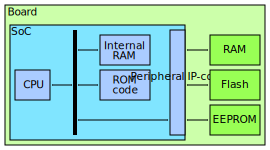
\includegraphics[scale=0.33]{images/board.pdf}
    \caption{Simplified view of Embedded board}
  \end{figure}
\end{frame}

\begin{frame}
  \frametitle{What is Bootloader?}
  \begin{columns}
    \column{0.5\textwidth}
      ROM code has limitations:
      \begin{itemize}
      \item Doesn't know about RAM
      \item Doesn't know board name
      \item Not flexible enough
      \end{itemize}
    \column{0.5\textwidth}
      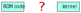
\includegraphics[scale=0.85]{images/bootloader1.pdf}
  \end{columns}
  \pause
  \bigskip
  \begin{columns}
    \column{0.5\textwidth}
      Bootloader to the rescue:
      \begin{itemize}
      \item Resides in flash (can be upgraded)
      \item Able to configure RAM
      \item Knows boot procedure
      \item Convenient features
      \end{itemize}
    \column{0.5\textwidth}
      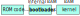
\includegraphics[scale=0.85]{images/bootloader2.pdf}
  \end{columns}
\end{frame}

\begin{frame}
  \frametitle{Why U-Boot?}
  \begin{columns}
    \column{0.5\textwidth}
      \begin{itemize}
      \item Bootloader for Embedded boards
        \begin{itemize}
        \item Popular for Android devices
        \item Adoption in automotive
        \end{itemize}
      \item GPLv2
      \item 13 architectures (consider ARM)
      \item \textasciitilde 300 boards
      \item Device drivers, lib routines
      \item Resembles Linux kernel a lot
      \item Scripting, extensive command set
      \end{itemize}
    \column{0.5\textwidth}
      \begin{figure}[ht]
      \begin{center}
        
\includegraphics[scale=2]{images/uboot-logo.pdf}
      \end{center}
      \end{figure}
  \end{columns}
\end{frame}

\begin{frame}
  \frametitle{U-Boot Features}
  \begin{itemize}
  \item Boots from various sources
  \item Boots various OSs
  \item Monitor (U-Boot shell)
    \begin{itemize}
    \item Commands
    \item Environment
    \end{itemize}
  \item 2 stage boot (SPL + U-Boot)
  \item ``Falcon'' mode (SPL only)
  \end{itemize}
\end{frame}

\begin{frame}
  \frametitle{Two Stage Boot}
  \begin{columns}
    \column{0.5\textwidth}
      \begin{figure}
        \centering
        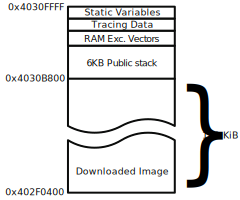
\includegraphics[scale=1]{images/sram.pdf}
        \caption{SRAM layout (from AM335x TRM)}
      \end{figure}
    \pause
    \column{0.5\textwidth}
      \begin{alertblock}{But bootloader is bigger!}
      For \textbf{\textsc{BeagleBone Black}}, \texttt{u-boot.img} is 391 KiB.
      \end{alertblock}
  \end{columns}
\end{frame}

\begin{frame}
  \frametitle{Two Stage Boot (cont'd)}
  \begin{columns}
    \column{0.5\textwidth}
      Let's add an intermediate stage (SPL):
      \begin{figure}
        \includegraphics[scale=0.29]{images/two-stage1.pdf}
      \end{figure}
      For \textbf{\textsc{BeagleBone Black}}:
      \begin{table}
        \begin{tabular}{@{} lr @{}}
          \toprule
          Stage & Size\\
          \midrule
          SPL & 75 KiB\\
          U-Boot & 391 KiB\\
          \bottomrule
        \end{tabular}
        \vspace*{-10mm} % to reduce too much whitespace after table
      \end{table}
    \pause
    \column{0.5\textwidth}
      \begin{center}
      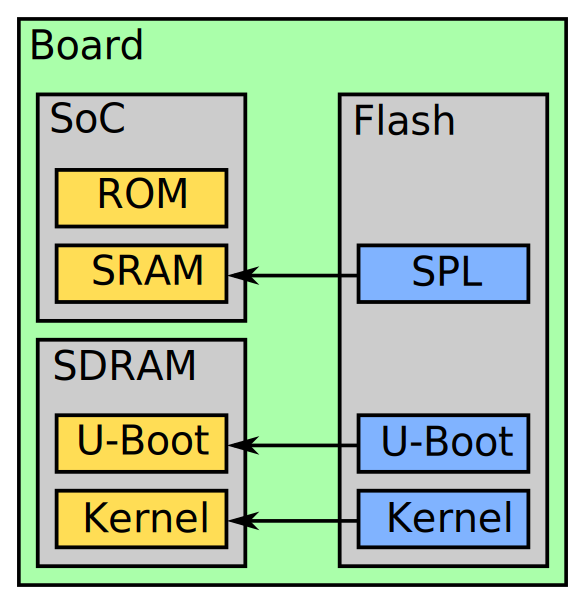
\includegraphics[scale=0.35]{images/two-stage2.pdf}
      \end{center}
  \end{columns}
\end{frame}

\begin{frame}
  \frametitle{Boot Sources}
  ROM code boot source is usually selected:
  \begin{itemize}
  \item Via \textbf{SYSBOOT} DIP switch
  \item By hard-wiring SYSBOOT lines (pull-up/pull-down)
  \item Using some USER button
  \item By inserting SD card (``Card Detect'' pin)
  \end{itemize}
  \pause
  U-Boot can boot kernel from:
  \begin{itemize}
  \item Flash devices (eMMC, SD card)
  \item Network boot (TFTP, NFS)
  \item Peripheral boot (USB, serial console)
  \end{itemize}
\end{frame}

\begin{frame}
  \frametitle{Flashing Methods}
  Most commonly used flashing methods:
  \begin{itemize}
  \item Via USB:
    \begin{itemize}
    \item fastboot (Android)
    \item DFU
    \end{itemize}
  \item Via SD card
  \end{itemize}
  \pause
  To unbrick the board (bad U-Boot on eMMC):
  \begin{itemize}
  \item Boot from SD card and re-flash
  \item Use JTAG
  \item USB peripheral boot
  \end{itemize}
\end{frame}

\begin{frame}[fragile]
  \frametitle{U-Boot Shell}
  \begin{itemize}
  \item U-Boot is a ``monitor'' program
  \item Command line interface
  \item A set of commands is implemented
  \item Resembles Bash (has scripting capabilities)
  \item Press ``Space'' to get into U-Boot shell
  \end{itemize}
  \pause
  Most commonly used commands:
  \begin{verbatim}
    bdinfo, bootm, bootz, crc32, dfu, dhcp, env,
    fastboot, fatload, fdt, gpt, i2c, md, mmc, mw,
    part, ping, reset, run, tftpboot, version, ...
  \end{verbatim}
\end{frame}

\begin{frame}[fragile]
  \frametitle{U-Boot Environment}
  \begin{columns}
    \column{0.5\textwidth}
      \begin{itemize}
      \item Keeps all U-Boot shell variables
      \item Just a set of strings in \texttt{key=value} format
      \end{itemize}
    \pause
    \column{0.5\textwidth}
      Set default environment:
      \begin{verbatim}
      => env default -f -a
      => env save
      \end{verbatim}
     \vspace*{-14mm} % to reduce too much whitespace after verbatim block
  \end{columns}
  \pause
  \bigskip
  \begin{center}
  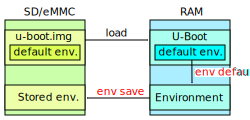
\includegraphics[scale=0.33]{images/env.pdf}
  \end{center}
\end{frame}

\begin{frame}[fragile]
  \frametitle{U-Boot Environment (cont'd)}
  \begin{verbatim}
  => env print

  board_name=A335BNLT
  board_rev=0A5A
  board_serial=1813BBBK4642
  bootargs=
  bootcmd=if test ${boot_fit} -eq 1; then ...
  fdtfile=am335x-boneblack.dtb
  findfdt=if test $board_name = A335BONE; then ...
  partitions=uuid_disk=${uuid_gpt_disk}; ...
  \end{verbatim}
\end{frame}

\begin{frame}[fragile]
  \frametitle{Use-case: Format eMMC}
  Using \texttt{gpt} command:
  \begin{verbatim}
  => gpt write mmc 1 $partitions
  \end{verbatim}
  \pause
  or Android way:
  \begin{verbatim}
  => fastboot 0
  $ fastboot oem format
  \end{verbatim}
  \pause
  \begin{itemize}
  \item Consider \alert{\texttt{\$partitions}} variable...
  \item Check with \texttt{part list mmc 1}
  \end{itemize}
\end{frame}

\begin{frame}[fragile]
  \frametitle{Use-case: Flashing eMMC}
  Via DFU:
  \begin{verbatim}
  => setenv dfu_alt_info $dfu_alt_info_emmc
  => dfu 0 mmc 1
  $ dfu-util -D MLO -a MLO.raw
  \end{verbatim}
  \pause
  Via fastboot (Android way):
  \begin{verbatim}
  => fastboot 0
  $ fastboot flash rootfs rootfs.img
  \end{verbatim}
\end{frame}

\begin{frame}[fragile]
  \frametitle{Use-case: Boot Linux}
  \begin{verbatim}
  => setenv mmcdev 1
  => setenv bootpart 1:2
  => run findfdt
  => run mmcboot
  \end{verbatim}
  \vspace*{-5mm} % to reduce too much whitespace after verbatim block
  \pause
  \begin{verbatim}
  mmcboot=
    mmc dev ${mmcdev}; mmc rescan;
    load mmc ${bootpart} ${loadaddr} /boot/zImage
    load mmc ${bootpart} ${fdtaddr} /boot/${fdtfile}
    setenv bootargs console=ttyO0,115200n8 root=... rw ...
    bootz ${loadaddr} - ${fdtaddr}
  \end{verbatim}
  \vspace*{-5mm} % to reduce too much whitespace after verbatim block
\end{frame}

\begin{frame}
  \frametitle{Boot Sequence}
  \texttt{do\_bootm\_linux()} calls:
  \begin{itemize}
    \item 1:
    \begin{itemize}
    \item \texttt{boot\_prep\_linux()}
    \item \texttt{boot\_setup\_linux()}
    \item \texttt{image\_setup\_libfdt()}
    \item Populates \texttt{/chosen} node with \texttt{bootargs},
          \texttt{initrd-start}, etc.
    \end{itemize}
    \item 2:
    \begin{itemize}
    \item \texttt{boot\_jump\_linux()}
    \item \texttt{kernel\_entry(0, machid, r2)}
    \item FDT blob address is passed to kernel via \texttt{r2}
    \end{itemize}
  \end{itemize}
\end{frame}

\begin{frame}
  \frametitle{Boot Methods Table}
      \begin{table}
        \begin{tabular}{@{} ll @{}}
          \toprule
          Boot method & Description\\
          \midrule
          SD card boot & \makecell[l]{
            - Unbrick the board               \\
            - Doesn't touch eMMC
          }                                   \\
          \hline
          eMMC boot & \makecell[l]{
            - Regular boot                    \\
            - Fastest and easiest for user
          }                                   \\
          \hline
          TFTP boot & \makecell[l]{
            - Network boot                    \\
            - Doesn't touch eMMC              \\
            - Volatile RootFS (RAM disk)
          }                                   \\
          \hline
          NFS boot & \makecell[l]{
            - Network boot                    \\
            - Transparent RootFS (from host)  \\
            - Useful for kernel development
          }                                   \\
          \bottomrule
        \end{tabular}
        \vspace*{-10mm} % to reduce too much whitespace after table
      \end{table}
\end{frame}

\section{IDE Considerations}

\begin{frame}[fragile]
  \frametitle{IDE for Kernel Development: Vim}
  \begin{columns}
    \column{0.5\textwidth}
    Pros:
    \begin{itemize}
      \item Very fast
      \item Available everywhere
      \item A lot of kernel hackers using it
    \end{itemize}
    \column{0.5\textwidth}
    Cons:
    \begin{itemize}
      \item Learning curve rather steep
      \item Some functionality is missing
      \item Requires some configuration
    \end{itemize}
  \end{columns}
  \bigskip
  Indexing example (simplified):
  \begin{verbatim}
make ARCH=arm SUBARCH=omap2 cscope tags
  \end{verbatim}
  Details: \href{https://stackoverflow.com/a/33682137/3866447}
                {https://stackoverflow.com/a/33682137/3866447}
\end{frame}

\begin{frame}
  \frametitle{IDE for Kernel Development: Vim (cont'd)}
  \begin{center}
    \includegraphics[scale=0.4]{images/vim.png}
  \end{center}
  \vspace*{-10mm} % to reduce too much whitespace after figure block
\end{frame}

\begin{frame}
  \frametitle{IDE for Kernel Development: Eclipse}
  \begin{columns}
    \column{0.5\textwidth}
    Pros:
    \begin{itemize}
      \item Easy to use
      \item Nice tools (indexing, macro unwrapping, etc)
    \end{itemize}
    \column{0.5\textwidth}
    Cons:
    \begin{itemize}
      \item Very slow
      \item Uses a lot of resources
      \item Not available on servers, etc.
    \end{itemize}
  \end{columns}
  \bigskip
  Be sure to configure CDT for kernel development.
  Details: \href{https://wiki.eclipse.org/HowTo\_use\_the\_CDT\_to\_navigate\_Linux\_kernel\_source}
                {https://wiki.eclipse.org/HowTo\_use\_the\_CDT\_to\_navigate\_Linux\_kernel\_source}
\end{frame}

\begin{frame}
  \frametitle{IDE for Kernel Development: Eclipse (cont'd)}
  \begin{center}
    \includegraphics[scale=0.35]{images/eclipse.png}
  \end{center}
  \vspace*{-10mm} % to reduce too much whitespace after figure block
\end{frame}

\begin{frame}
  \frametitle{IDE for Kernel Development: Other Choices}
  Other possible IDEs:
  \begin{itemize}
    \item Emacs
    \item KDevelop
    \item QtCreator
  \end{itemize}

  Kernel source web-browser (very useful):
  \begin{itemize}
    \item \href{elixir.bootlin.com}{elixir.bootlin.com}
  \end{itemize}
\end{frame}

\begin{frame}[standout]
  Questions so far?
\end{frame}

\begin{frame}[standout]
  Take Five
\end{frame}

\section{Workshop: Bringing up the BBB}

\subsection{TC Infrastructure}

\begin{frame}
  \frametitle{Short Quiz}
  \begin{enumerate}
    \item Who didn't manage to build all the SW?
    \item Who doesn't have a laptop along?
  \end{enumerate}
\end{frame}

\begin{frame}
  \frametitle{Training Centre Infrastructure}

  Training Centre PC info:
  \begin{itemize}
    \item Press F9 on boot (show boot menu)
    \item Select second drive (TS64GSSD370S, 64 GB)
    \item Login: Lin-Ker
    \item Password: 123
  \end{itemize}

  What does it have?
  \begin{itemize}
    \item Ubuntu 18.04, internet connection, prepared environment
    \item Toolchains (\texttt{/opt/*})
    \item U-Boot, Linux kernel, BusyBox (see \texttt{\textasciitilde/repos/*})
    \item \textbf{Missing}: TRM, datasheet, schematic, BBB instructions guide
  \end{itemize}
\end{frame}

\begin{frame}
  \frametitle{Training Centre Infrastructure (cont'd)}
  Notes:
  \begin{itemize}
    \item Better to use home laptop to keep the single environment
    \item We only have one card reader :(
  \end{itemize}
\end{frame}

\subsection{Hardware Concerns}

\begin{frame}
  \frametitle{Hardware Equipment}
  \begin{itemize}
    \item \textbf{The board}: BeagleBone Black Rev C
    \item \textbf{Serial cable}: TTL-232R-3V3
    \item \textbf{OTG USB cable}: mini-USB to USB
    \item \textbf{micro-SD card + adapter}: 8 GB, class 10
    \item \textbf{Ethernet patch cord}: for network boot and networking tasks
    \item \textbf{Development kit}: a set of hardware, will be used later
  \end{itemize}
\end{frame}

\begin{frame}
  \frametitle{ESD Safety Note}
  \begin{columns}
    \column{0.5\textwidth}
      \begin{center}
        \includegraphics[scale=0.05]{images/esd01.png}
      \end{center}
      \begin{itemize}
        \item Discharge before touching
        \item Use ESD mat and wrist strap
        \item Don't wear ESD unsafe clothes
        \item Remove power plug before touching
      \end{itemize}
    \column{0.5\textwidth}
      \begin{center}
        \includegraphics[scale=0.55]{images/esd03.jpg}
      \end{center}
  \end{columns}
\end{frame}

\subsection{Connectivity}

\begin{frame}
  \frametitle{Connectivity: Overview}
  \alert{Don't do this just yet!}
  \begin{itemize}
  \item Connect mini-USB cable
    \begin{itemize}
    \item Powering the board (low consumption use-case)
    \item Flashing (\texttt{fastboot}, \texttt{dfu-util})
    \end{itemize}
  \item Connect serial console cable (white dot = black wire = GROUND)
    \begin{itemize}
    \item Will be used via \texttt{minicom} tool
    \end{itemize}
  \item Insert SD card to the slot (once it's flashed with software)
  \end{itemize}
\end{frame}

\begin{frame}
  \frametitle{Connectivity: Serial Console}
  \begin{columns}
    \column{0.5\textwidth}
    \begin{figure}
      \centering
      \includegraphics[scale=0.5]{images/bbb-serial.png}
      \caption{BeagleBone Black serial connection}
    \end{figure}
    \column{0.5\textwidth}
    \begin{figure}
      \centering
      \includegraphics[scale=0.3]{images/ftdi-cable.png}
      \caption{TTL-232R-3V3 FTDI cable}
    \end{figure}
  \end{columns}
\end{frame}

\begin{frame}
  \frametitle{Connectivity: Serial Console (cont'd)}
  \begin{itemize}
    \item Board uses UART port (TTL levels, 3.3V) to communicate:
    \begin{itemize}
      \item Rx line for receiving characters from host
      \item Tx line for transceiving characters to host
    \end{itemize}
    \item Chip in adapter cable converts UART <-> USB
    \begin{itemize}
      \item FT232R (FTDI): reliable, recommended
      \item PL2303: cheap alternative
    \end{itemize}
    \item Chip driver exposes \texttt{/dev/ttyUSB} file (char device)
    \item \texttt{minicom} (or similar tool) allows user to interact with board
          via \texttt{/dev/ttyUSB}
  \end{itemize}
\end{frame}

\begin{frame}
  \frametitle{Connectivity: Client USB (OTG)}
  \begin{figure}
    \centering
    \includegraphics[scale=0.4]{images/bbb-otg.png}
    \caption{BeagleBone Black USB connection}
  \end{figure}
\end{frame}

\begin{frame}[fragile]
  \frametitle{Configure and Run \texttt{minicom}}
  \begin{itemize}
    \item Run minicom configuration:
    \begin{verbatim}
$ sudo minicom -s
    \end{verbatim}
    \item Select ``Serial port setup'' menu item and choose next settings:
      \begin{itemize}
        \item Serial Device: \texttt{/dev/ttyUSB0}
        \item Bps/Par/Bits: 115200 8N1
	\item Hardware Flow Control: \alert{\textbf{No}}
      \end{itemize}
    \item Then select ``Save setup as dfl'' and ``Exit from Minicom''
    \item Run minicom:
    \begin{verbatim}
$ sudo minicom
    \end{verbatim}
  \end{itemize}
\end{frame}

\begin{frame}
  \frametitle{Configure and Run \texttt{minicom} (cont'd)}
  \begin{figure}
    \centering
    \includegraphics[scale=0.6]{images/minicom.png}
    \caption{Terminal with minicom}
  \end{figure}
  \vspace*{-5mm} % to reduce too much whitespace after figure block
\end{frame}

\subsection{Running RootFS from SD Card}

\begin{frame}[fragile]
  \frametitle{Formatting SD Card (page 1)}
  \begin{itemize}
    \item Insert your SD card in your laptop (use adapter)
    \item Locate SD card device file (should be \texttt{/dev/mmcblk0}):
      \begin{verbatim}
$ sudo dmesg | tail
$ sudo fdisk -l
      \end{verbatim}
    \item Unmount SD card (mounted automatically by Ubuntu):
      \begin{verbatim}
$ sudo umount /dev/mmcblk0p1
$ sudo umount /dev/mmcblk0p2
      \end{verbatim}
    \item Clear SD card MBR:
      \begin{verbatim}
$ sudo dd if=/dev/zero of=/dev/mmcblk0 bs=1M count=1
      \end{verbatim}
  \end{itemize}
  \vspace*{-5mm} % to reduce too much whitespace after verbatim block
\end{frame}

\begin{frame}[fragile]
  \frametitle{Formatting SD Card (page 2)}
  \begin{itemize}
    \item Create new partition table:
      \begin{verbatim}
$ sudo sfdisk /dev/mmcblk0 << EOF
2048,100M,0x0c,*
,,L,-
EOF
      \end{verbatim}
    \item Format both partitions:
      \begin{verbatim}
$ sudo mkfs.vfat -F 32 -n "boot" /dev/mmcblk0p1
$ sudo mkfs.ext4 -F -L "rootfs"  /dev/mmcblk0p2
      \end{verbatim}
  \end{itemize}
\end{frame}

\begin{frame}[fragile]
  \frametitle{Formatting SD Card (page 3)}
  \begin{itemize}
    \item Check new partitions:
      \begin{verbatim}
$ sudo fdisk -l
      \end{verbatim}
    \item You should see something like this:
      \begin{verbatim}
Device          Boot  Start  Size  Id  Type
/dev/mmcblk0p1  *      2048  100M   c  W95 FAT32 (LBA)
/dev/mmcblk0p2       206848  14.9G 83  Linux
      \end{verbatim}
  \end{itemize}
\end{frame}

\begin{frame}[fragile]
  \frametitle{Prepare Bootable SD Card (page 1)}
  \begin{itemize}
    \item Unmount SD card (mounted automatically by Ubuntu):
      \begin{verbatim}
$ sudo umount /dev/mmcblk0p1
$ sudo umount /dev/mmcblk0p2
      \end{verbatim}
    \item Mount partitions:
      \begin{verbatim}
$ sudo mkdir /mnt/{boot,rootfs}
$ sudo mount /dev/mmcblk0p1 /mnt/boot
$ sudo mount /dev/mmcblk0p2 /mnt/rootfs
      \end{verbatim}
    \item Check that partitions mounted properly:
      \begin{verbatim}
$ mount | grep mmcblk
      \end{verbatim}
  \end{itemize}
  \vspace*{-5mm} % to reduce too much whitespace after verbatim block
\end{frame}

\begin{frame}[fragile]
  \frametitle{Prepare Bootable SD Card (page 2)}
  \begin{itemize}
    \item Copy U-Boot files to SD card (``boot'' partition):
      \begin{verbatim}
$ cd ~/repos/u-boot
$ sudo cp MLO u-boot.img /mnt/boot
      \end{verbatim}
    \item Copy rootfs files to SD card (``rootfs'' partition):
      \begin{verbatim}
$ cd ~/repos/busybox/_install
$ sudo cp -R . /mnt/rootfs
      \end{verbatim}
  \end{itemize}
\end{frame}

\begin{frame}[fragile]
  \frametitle{Prepare Bootable SD Card (page 3)}
  \begin{itemize}
    \item Unmount SD card:
      \begin{verbatim}
$ sudo umount /mnt/boot
$ sudo umount /mnt/rootfs
      \end{verbatim}
    \item Remove your SD card from your laptop
  \end{itemize}
\end{frame}

\begin{frame}[fragile]
  \frametitle{Booting from SD Card}
  \begin{itemize}
    \item Unplug mini-USB cable from the board
    \item Insert SD card in board's slot
    \item Press and hold \texttt{USER/BOOT} button
    \item Plug power cable and mini-USB cable back to board
    \item Release \texttt{USER/BOOT} button
    \item BusyBox will be loaded from SD card
  \end{itemize}
\end{frame}

\section*{Assignments}

\begin{frame}
  \frametitle{Assignment \#1}
  \begin{itemize}
    \item Finish up the whole BBB guide:
      \begin{itemize}
        \item Do all kinds of boot, using 3rd chapter (eMMC boot, TFPT boot,
              NFS boot)
        \item Use previously built software (from lecture 1 assignment)
      \end{itemize}
    \item Proof:
      \begin{itemize}
        \item Send me screenshots that prove eMMC boot works for you
        \item Send me screenshots that prove NFS boot works for you
      \end{itemize}
  \end{itemize}
\end{frame}

\begin{frame}
  \frametitle{Assignment \#2}
  \begin{itemize}
    \item Install and configure IDE of your choice (use links from slides)
    \item In your IDE (work dir must be the kernel source dir):
      \begin{itemize}
      \item Open \texttt{init/main.c} file
      \item Find \texttt{start\_kernel()} function implementation
      \item In \texttt{start\_kernel()}, look for \texttt{setup\_arch()} call
      \item Jump to \texttt{setup\_arch()} (using IDE capabilities)
      \item Get back to \texttt{start\_kernel()} (using IDE capabilities)
      \item Find where \texttt{start\_kernel()} is being called from (using IDE
            capabilities)
      \end{itemize}
    \item Proof: send me screenshot that shows your configured IDE
  \end{itemize}
\end{frame}

\begin{frame}[standout]
  Thank you!
\end{frame}

\section*{Appendix: Abbreviations}

\begin{frame}
  \frametitle{Abbreviations}
  \begin{itemize}
    \item BBB - BeagleBone Black
    \item DFU - Device Firmware Upgrade
    \item DTB - Device Tree Blob
    \item eMMC - Embedded MMC (MultiMedia Card)
    \item ESD - Electrostatic Discharge
    \item FDT - Flattened Device Tree (the same as DTB)
    \item FTDI - Future Technology Devices International
    \item GPIO - General Purpose Input Output
    \item GPT - GUID Partition Table
    \item IDE - Integrated Development Environment
    \item LED - Light-Emitting Diode
  \end{itemize}
\end{frame}

\begin{frame}
  \frametitle{Abbreviations (cont'd)}
  \begin{itemize}
    \item MBR - Master Boot Record
    \item MLO - MMC Loader (the same as SPL)
    \item NFS - Network File System
    \item OTG - USB On-The-Go
    \item PCB - Printed Circuit Board
    \item PHY - Physical layer chip
    \item PMIC - Power Management IC (Integrated Circuit)
    \item RootFS - Root File System
    \item SD card - Secure Digital card
    \item SoC - System on Chip
    \item SPL - Secondary Program Loader
  \end{itemize}
\end{frame}

\begin{frame}
  \frametitle{Abbreviations (cont'd)}
  \begin{itemize}
    \item TFTP - Trivial File Transport Protocol
    \item TRM - Technical Reference Manual
    \item TTL - Transistor-to-Transistor Logic
    \item UART - Universal Asynchronous Receiver-Transmitter
  \end{itemize}
\end{frame}

\end{document}
